% Origen: sección "Apéndice" de Secciones/PI - Hardware empleado.md
\chapter{Complementos del hardware empleado}
\label{C:ap-hw}

% Figuras de este apéndice + las compartidas.
\graphicspath{{figs/apendices/}{figs/comunes/}}

\section{Criterios de selección de plataforma de HW}
\label{S:ap-hw-criterios}

% Ocupa más de una página: longtable, para que se corte entre filas.
{\small
\begin{longtable}{|>{\raggedright\arraybackslash}p{0.27\textwidth}%
  |>{\raggedright\arraybackslash}p{\dimexpr0.73\textwidth-4\tabcolsep-3\arrayrulewidth\relax}|}
\caption[Criterios de selección de plataforma de HW]{%
Criterios de selección de plataforma de HW. Extraída del
ZynqBook~\citecap{Crockett2014}{4}.\label{t:ap-hw-criterios}} \\
\hline
\encabezado \textbf{Categoría} & \textbf{Factores} \\ \hline
\endfirsthead
\hline
\encabezado \textbf{Categoría} & \textbf{Factores} \\ \hline
\endhead
\textbf{Capacidades del dispositivo} & Rendimiento del procesador\newline
  Rendimiento de la lógica\newline
  Rendimiento de la memoria\newline
  Soporte para aritmética de alta velocidad\newline
  Soporte para E/S y comunicaciones\newline
  Funciones de seguridad y soporte para arranque seguro\newline
  Ancho de banda entre procesador y lógica\newline
  Latencia entre procesador y lógica \\ \hline
\textbf{Factores comerciales} & Lista de materiales (BOM)\newline
  Costos de desarrollo\newline
  Integración (y costos implícitos)\newline
  Longevidad de disponibilidad del dispositivo y soporte técnico\newline
  Calidad y confiabilidad\newline
  Facilidad (costo) de actualizaciones en campo \\ \hline
\textbf{Diseño y desarrollo} & Tiempo de salida al mercado\newline
  Flujos de diseño rápidos, cómodos y confiables\newline
  Verificación integrada\newline
  Integración con otras herramientas de desarrollo\newline
  Soporte para flujos de diseño en equipo\newline
  Soporte para reutilización de diseños\newline
  Soporte para formatos de diseño estándar de la industria\newline
  Soporte para los métodos de entrada de diseño deseados\newline
  Documentación y soporte técnico \\ \hline
\textbf{Características físicas del dispositivo} & Tamaño físico\newline
  Consumo de potencia\newline
  Facilidad de integración y complejidad resultante del PCB\newline
  Conectividad\newline
  Robustez\newline
  Sensibilidad a la radiación\newline
  Rango de temperatura soportado \\ \hline
\textbf{Flexibilidad} & Escalabilidad \emph{(hay dispositivos más grandes y más
  chicos que se pueden adoptar con poco o ningún retrabajo)}\newline
  Portabilidad \emph{(diseños en formatos estándar que se pueden migrar
  desde/hacia otras plataformas)}\newline
  Reprogramabilidad \emph{(capacidad de cambiar la funcionalidad en campo o
  incluso dinámicamente en tiempo de ejecución)}\newline
  Facilidad de particionado \emph{(capacidad de repartir la funcionalidad entre
  hardware y software)}\newline
  Expansibilidad \emph{(facilidad para integrar nueva funcionalidad)} \\ \hline
\end{longtable}}

\section{Detalles de las CLB}
\label{S:ap-hw-clb}

Cada \emph{slice}, a su vez, contiene~\cite{UG474}:
\begin{itemize}
  \item \textbf{4 Look-Up Tables (LUT) de 6 entradas.} Una LUT es una memoria
    SRAM de 64 bits que almacena la tabla de verdad de una función lógica
    arbitraria de hasta 6 variables: configurar la FPGA es, literalmente,
    escribir esas tablas. Cada LUT tiene \textbf{doble salida} (O5/O6) y puede
    usarse como una LUT de 6 entradas o como dos LUT de 5 entradas con las
    entradas compartidas, lo que permite empaquetar dos funciones pequeñas en el
    mismo recurso.
  \item \textbf{8 flip-flops tipo D}, el bloque de memoria mínima sincrónica al
    reloj. Admiten \emph{clock enable} (CE) y \emph{set/reset} (SR). Los 8
    flip-flops de un \emph{slice} comparten el mismo reloj, el mismo CE y el
    mismo SR, esto se suele llamar \emph{control set}. Un diseño con muchos CE
    distintos no puede empaquetar bien y termina ocupando más \emph{slices} de
    los que su cuenta de lógica sugiere.
  \item \textbf{Lógica de acarreo dedicada (CARRY4).} Cuatro bits de cadena de
    acarreo con ruteo propio, vertical y mucho más rápido que la interconexión
    general. Es lo que hace que un sumador en FPGA sea eficiente: sin ella, cada
    acarreo pagaría un salto por la matriz de conmutación.
  \item \textbf{Multiplexores dedicados (F7, F8)}, que combinan las salidas de
    varias LUT para construir funciones de 7 u 8 entradas sin gastar
    interconexión.
\end{itemize}

\section{Detalles de las entradas analógicas rápidas}
\label{S:ap-hw-entradas}

En la Fig.~\ref{f:ap-hw-frontend} aparece el front-end analógico de las entradas
rápidas.

\begin{figure}[H]
\centering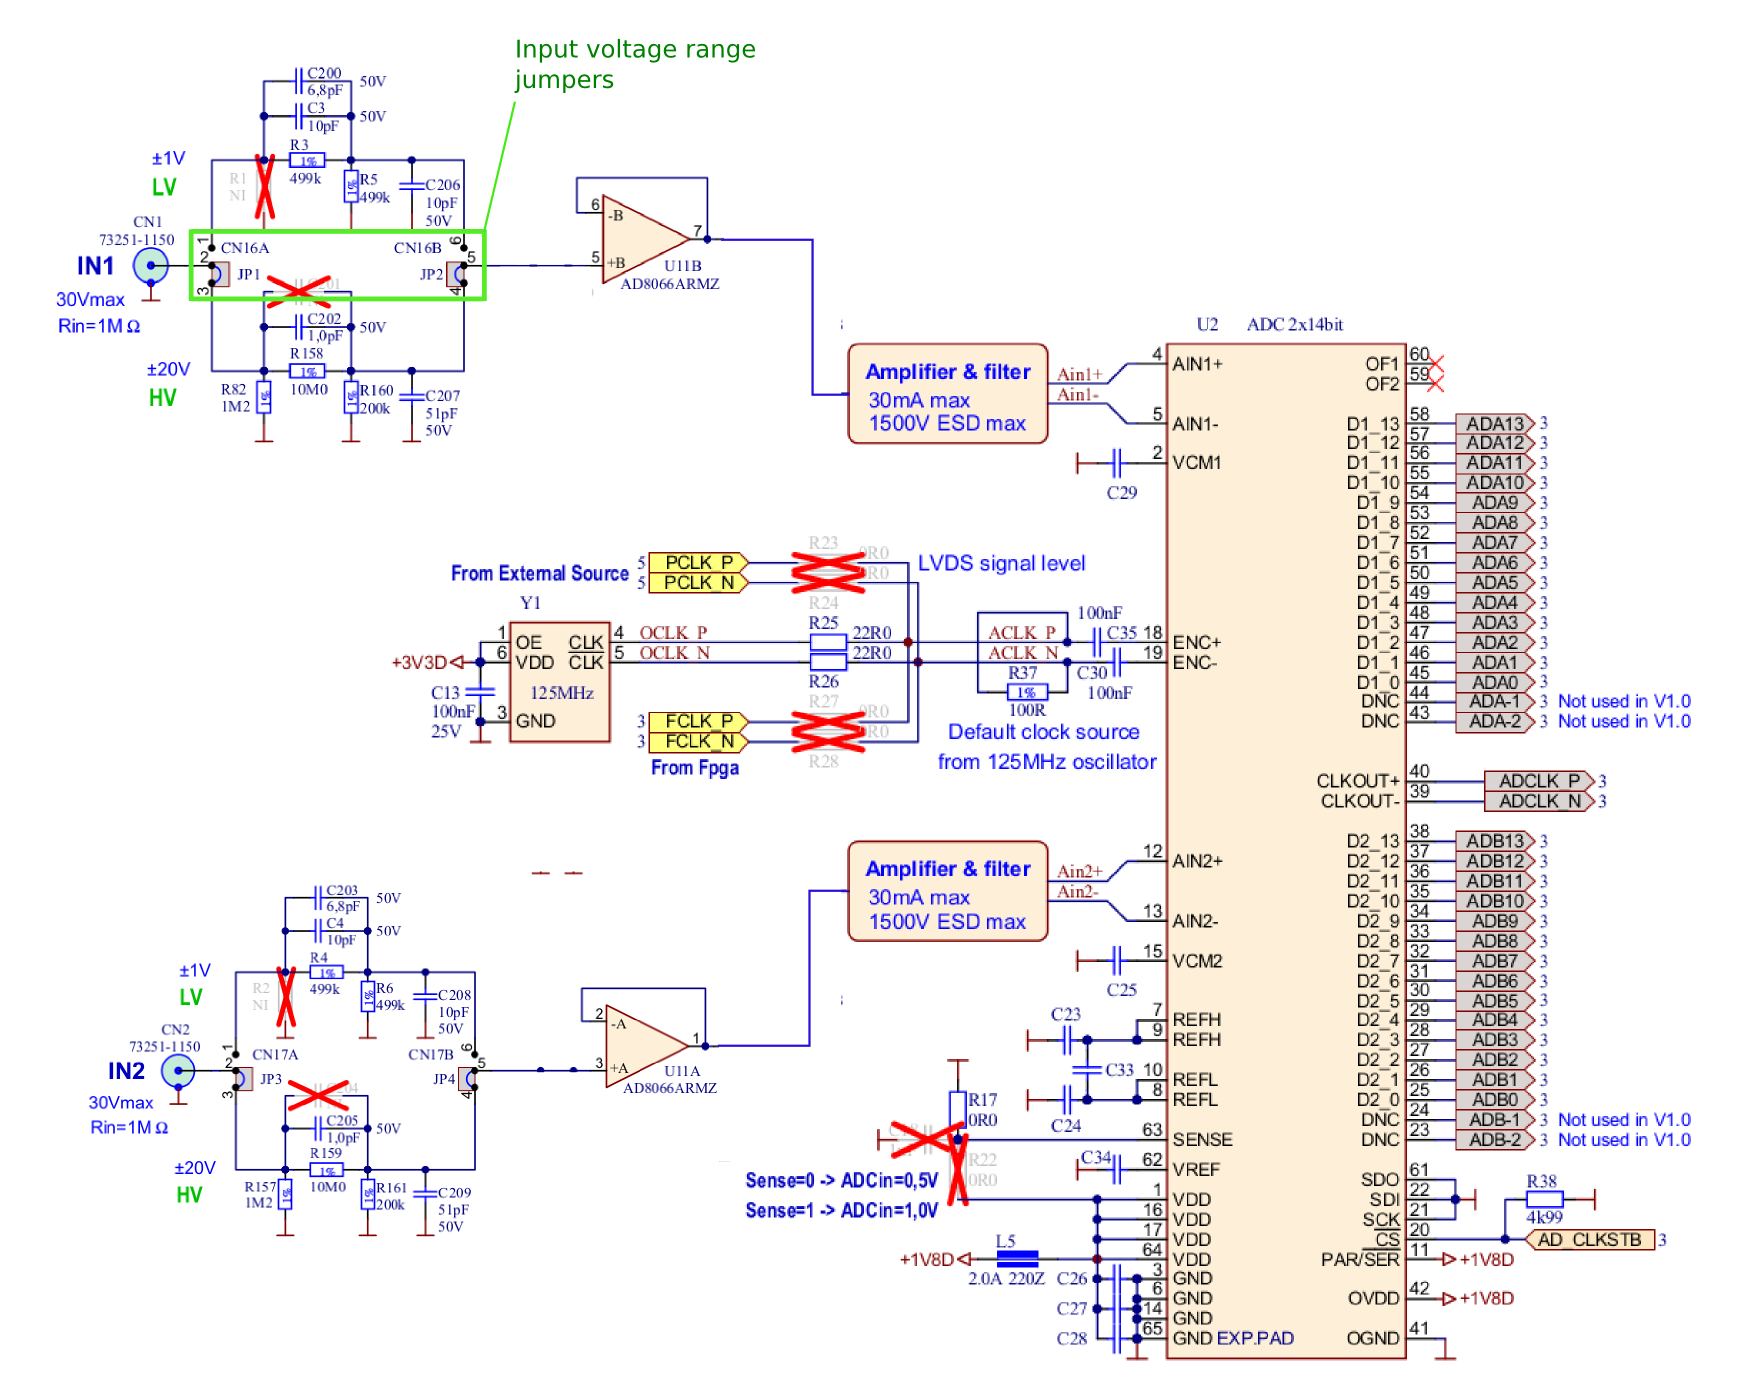
\includegraphics{apB_frontend_pitaya}
\caption[Front-end analógico de las entradas rápidas]{%
Front-end analógico de las entradas de la plataforma: divisor con los jumpers
LV/HV, un buffer (AD8066) y una etapa de amplificación y filtrado antes del ADC.
Extraído del esquemático de Red Pitaya~\cite{RedPitayaSchematics}.
\label{f:ap-hw-frontend}}
\end{figure}

En la Tabla~\ref{t:ap-hw-crosstalk} se presenta la diafonía (\emph{crosstalk})
máxima entre los dos canales de entrada, para cada combinación de jumpers LV/HV.

\begin{table}[H]
\centering
\caption[Diafonía entre los canales IN1 e IN2]{%
Diafonía máxima entre los canales IN1 e IN2 en todas las
configuraciones~\cite{RedPitayaDocs}.\label{t:ap-hw-crosstalk}}
\small
\begin{tabular}{|c|c|c|c|c|}
\hline
\encabezado & \multicolumn{2}{c|}{\textbf{Hasta 30~MHz}}
  & \multicolumn{2}{c|}{\textbf{Por encima de 30~MHz}} \\ \hline
\encabezado \textbf{IN2 \textbackslash{} IN1} & \textbf{LV} & \textbf{HV}
  & \textbf{LV} & \textbf{HV} \\ \hline
\textbf{LV} & $>$55~dB & 50~dB & 40~dB & 40~dB \\ \hline
\textbf{HV} & $>$55~dB & $>$50~dB & $>$40~dB & $>$35~dB \\ \hline
\end{tabular}
\end{table}

En la Fig.~\ref{f:ap-hw-respuesta-in} se presenta la curva de la documentación
oficial de Red Pitaya.

\begin{figure}[H]
\centering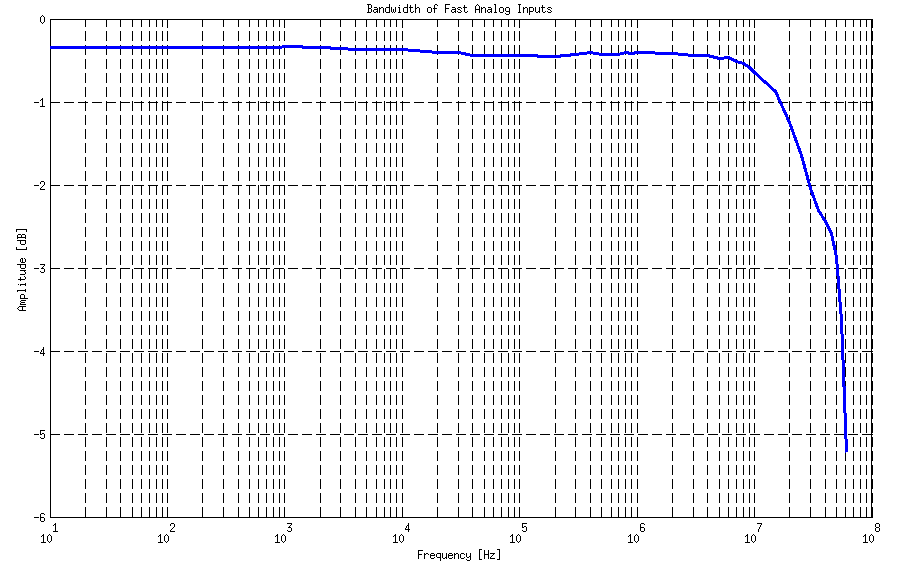
\includegraphics{apB_respuesta_frontend_in}
\caption[Respuesta en frecuencia del front-end de entrada]{%
Módulo de la respuesta en frecuencia del front-end de entrada analógica, de la
documentación de Red Pitaya~\cite{RedPitayaFastIn}. La caída de $-3$~dB está en
aproximadamente 50~MHz.\label{f:ap-hw-respuesta-in}}
\end{figure}

\section{Detalles de la salida analógica rápida: DAC}
\label{S:ap-hw-dac}

La STEMlab 125-14 tiene dos salidas analógicas rápidas, OUT1 y OUT2,
alimentadas por un único conversor digital-analógico (DAC) dual, el AD9767 de
Analog Devices~\cite{AD9767}. Cada salida del conversor pasa por una etapa de
amplificación y filtrado antes del conector SMA (Fig.~\ref{f:ap-hw-dac-etapa}).
En este proyecto OUT1 la maneja el generador de pulsos \codigo{gen\_pulsos}, en
el lugar que dejó libre el generador arbitrario (ASG) de Red Pitaya, para las
pruebas de generación interna por el canal analógico
(Fig.~\ref{f:res-conexion-in-out}).

\begin{figure}[H]
\centering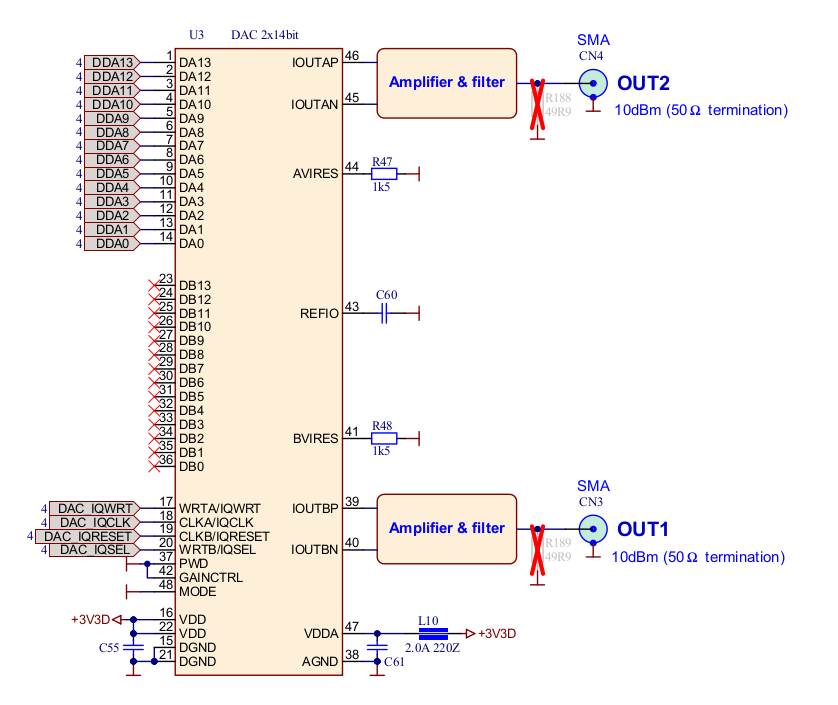
\includegraphics{apB_dac_etapa_salida}
\caption[Conexión del DAC AD9767 en la STEMlab 125-14]{%
Conexión del DAC AD9767 en la STEMlab 125-14, de la documentación de Red
Pitaya~\cite{RedPitayaFastOut}. Las resistencias serie de 49.9~$\Omega$ (R188 y
R189) están sin montar.\label{f:ap-hw-dac-etapa}}
\end{figure}

En la Tabla~\ref{t:ap-hw-salida-rapida} se presentan las características de la
salida según la documentación de Red Pitaya.

\begin{table}[H]
\centering
\caption[Características de las salidas analógicas rápidas]{%
Características de las salidas analógicas rápidas de la STEMlab 125-14, según
la documentación de Red Pitaya~\cite{RedPitayaFastOut}.
\label{t:ap-hw-salida-rapida}}
\small
\begin{tabularx}{\textwidth}{|>{\raggedright\arraybackslash}p{0.27\textwidth}|>{\raggedright\arraybackslash}X|}
\hline
\encabezado & \textbf{Valor} \\ \hline
Canales & 2 (OUT1, OUT2), conector SMA \\ \hline
Tasa de actualización & 125~MS/s por canal \\ \hline
Resolución & 14 bit \\ \hline
Acoplamiento & DC \\ \hline
Rango de salida & ±1~V sobre 50~$\Omega$ \\ \hline
Carga especificada & \textbf{50~$\Omega$}: las salidas sin uso se terminan, y
  una carga de alta impedancia se conecta con una T y 50~$\Omega$ en paralelo
  \\ \hline
Ancho de banda & 50~MHz ($-3$~dB) en la medición; la página de la placa
  declara DC--60~MHz~\cite{RedPitayaDocs} \\ \hline
Límite de \emph{slew rate} & 200~V/µs \\ \hline
Potencia a fondo de escala & $>$~9~dBm; 9.5~dBm típicos con una senoide de
  1~MHz (±1~V de pico sobre 50~$\Omega$ serían 10~dBm) \\ \hline
Armónicos a 8~dBm & $-51$, $-49$, $-48$ y $-53$~dBc a 1, 10, 20 y 45~MHz
  \\ \hline
Errores sin calibrar & offset $<$ 5~\% FS · ganancia $<$ 5~\% \\ \hline
Codificación & offset binary de \textbf{pendiente negativa}, como el ADC: el top
  convierte el complemento a 2 con
  \codigo{\{dac[13], \textasciitilde{}dac[12:0]\}} \\ \hline
Interfaz con la PL & bus paralelo de 14 bits \codigo{LVCMOS33} \\ \hline
\end{tabularx}
\end{table}

Dos números de la tabla limitan los pulsos rápidos. Con 200~V/µs, un escalón de
fondo de escala (2~V) tarda al menos 10~ns, algo más de una muestra, y una
senoide de amplitud $A$ deja de ser lineal por encima de $f = SR/(2\pi A)$: unos
32~MHz para $A = 1$~V. Por eso, según la documentación, el \emph{slew rate} es
el que limita la potencia de salida a fondo de escala. El ancho de banda, por su
parte, redondea los flancos: un sistema de primer orden con su frecuencia de
corte en 50~MHz tiene un tiempo de subida (10--90~\%) de
$0{,}35/f_{-3\,\text{dB}} \approx 7$~ns.

\subsection{El conversor AD9767}
\label{S:ap-hw-ad9767}

El AD9767 es un DAC con salida en corriente. Cada canal entrega un par de
corrientes complementarias, cuya suma es la corriente de fondo de escala
$I_{FS}$. Esa corriente la fijan una resistencia externa $R_{SET}$, en el pin
FSADJ, y la referencia interna de 1.20~V:
\begin{equation}
  I_{FS} = 32\,\frac{V_{REF}}{R_{SET}}, \qquad
  I_{OUTA} = I_{FS}\,\frac{\text{código}}{2^{14}}, \qquad
  I_{OUTB} = I_{FS}\,\frac{2^{14}-1-\text{código}}{2^{14}}
  \label{e:ap-hw-ad9767}
\end{equation}

La etapa de amplificación de la placa convierte esa corriente diferencial en la
tensión de salida. Las características principales del conversor, según su hoja
de datos, se presentan en la Tabla~\ref{t:ap-hw-ad9767}.

\begin{table}[H]
\centering
\caption[Características del DAC AD9767]{%
Características del AD9767 según su hoja de datos~\cite{AD9767}, con
$I_{FS}$~=~20~mA y salida diferencial.\label{t:ap-hw-ad9767}}
\small
\begin{tabularx}{\textwidth}{|>{\raggedright\arraybackslash}p{0.35\textwidth}|>{\raggedright\arraybackslash}X|}
\hline
\encabezado & \textbf{Valor} \\ \hline
Resolución y tasa máxima & 14 bit, 125~MSPS \\ \hline
Salida & corriente complementaria, $I_{FS}$ de 2 a 20~mA \\ \hline
Rango de cumplimiento (\emph{compliance}) & $-1.0$ a $+1.25$~V \\ \hline
INL / DNL a 25~°C & ±1.5 / ±1.0~LSB típicos; ±3.5 / ±2.5~LSB máximos \\ \hline
Apareamiento de ganancia entre canales & ±0.1~\% FSR típico \\ \hline
Establecimiento al 0.1~\% & 35~ns \\ \hline
Subida y bajada (10--90~\%) & 2.5~ns \\ \hline
Impulso de \emph{glitch} & 5~pV$\cdot$s \\ \hline
SFDR a 125~MSPS & 67~dBc con $f_{out}$~=~25~MHz · 70~dBc con 40~MHz \\ \hline
\end{tabularx}
\end{table}

Los 35~ns de establecimiento son unas 4 muestras: un escalón del DAC no queda
dentro del 0.1~\% de su valor final hasta la cuarta o quinta muestra, aparte de
lo que agregue la etapa de salida.

\subsection{Respuesta en frecuencia e impedancia de salida}
\label{S:ap-hw-respuesta-dac}

En la Fig.~\ref{f:ap-hw-dac-respuesta} se presenta la respuesta en frecuencia
de la salida medida por Red Pitaya, con OUT1 a 0~dBm y la otra salida y las dos
entradas terminadas en 50~$\Omega$. Es plana dentro de medio dB hasta unos
35~MHz, con un pequeño sobrepico (+0.3~dB) cerca de 25~MHz, y cae 3~dB en unos
50~MHz.

% Las dos curvas van juntas, lado a lado: por separado la segunda quedaba sola
% en una página al final del apéndice. Cada una mantiene su número y epígrafe.
\begin{figure}[H]
\begin{minipage}[t]{0.49\textwidth}
\captionsetup{width=0.95\linewidth}
\centering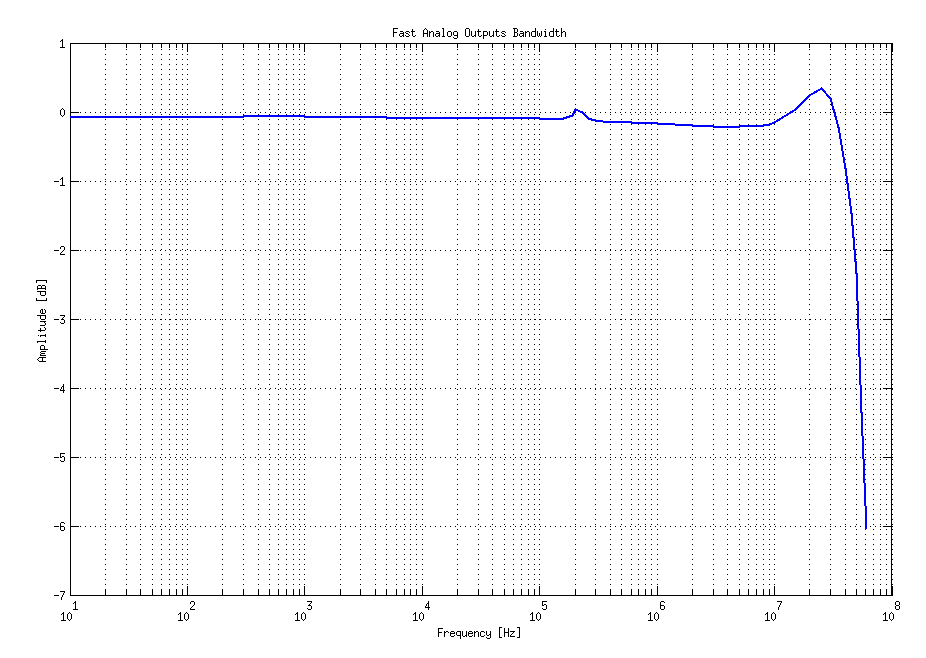
\includegraphics{apB_dac_respuesta_frecuencia}
\caption[Respuesta en frecuencia de las salidas rápidas]{%
Módulo de la respuesta en frecuencia de las salidas rápidas, de la
documentación de Red Pitaya~\cite{RedPitayaFastOut}.
\label{f:ap-hw-dac-respuesta}}
\end{minipage}\hfill
\begin{minipage}[t]{0.49\textwidth}
\captionsetup{width=0.95\linewidth}
\centering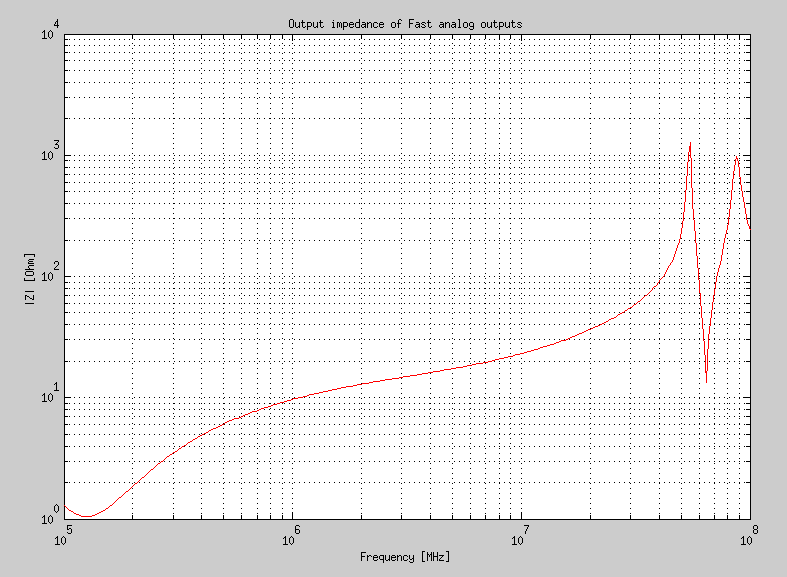
\includegraphics{apB_dac_impedancia}
\caption[Impedancia de salida de las salidas rápidas]{%
Módulo de la impedancia de salida de las salidas rápidas, de la documentación
de Red Pitaya~\cite{RedPitayaFastOut}. El eje horizontal está en Hz.
\label{f:ap-hw-dac-impedancia}}
\end{minipage}
\end{figure}

La salida no es una fuente de 50~$\Omega$: el esquemático prevé una resistencia
serie de 49.9~$\Omega$ por canal (R188 y R189), pero está sin montar. La
impedancia de salida, en la Fig.~\ref{f:ap-hw-dac-impedancia}, es de alrededor
de 1~$\Omega$ a 100~kHz, sube a unos 10~$\Omega$ en 1~MHz y a unos 20~$\Omega$
en 10~MHz, y por encima de los 40~MHz presenta resonancias de hasta
$\sim$1~k$\Omega$. Por eso Red Pitaya pide terminar las salidas en 50~$\Omega$:
con un coaxial sin terminar en el otro extremo, la línea queda desadaptada en
las dos puntas y la señal rebota en el cable. Por la misma razón, la amplitud
sin carga no se duplica, como pasaría con una fuente de 50~$\Omega$.

La caracterización del canal OUT1 $\rightarrow$ IN1 que usamos en las pruebas de
generación interna por el canal analógico se presenta en la
Sec.~\ref{S:res-setup-interna}.

% Las figuras y tablas son más largas que el texto: sin el \clearpage flotan
% detrás de las referencias.
\clearpage
\bibliografiacapitulo

%%% Local Variables:
%%% mode: latex
%%% TeX-master: "template"
%%% End:
